% ============================================================
% 第17章 勾股定理 — 人教版八年级下册
% 编译命令：xelatex -interaction=nonstopmode 第17章_勾股定理.tex
% ============================================================
\documentclass[12pt, a4paper]{ctexart}
\usepackage[margin=2.2cm]{geometry}
\usepackage{amsmath, amssymb}
\usepackage{enumitem}
\usepackage{tcolorbox}
\usepackage{booktabs}
\usepackage{array}
\usepackage{fancyhdr}
\usepackage{xcolor}
\usepackage{tikz}
\usepackage{hyperref}
\usepackage{graphicx}
\usepackage{multirow}
\usepackage{pgfplots}
\pgfplotsset{compat=1.18}

% 颜色定义
\definecolor{mainblue}{RGB}{41, 98, 168}
\definecolor{lightblue}{RGB}{230, 240, 255}
\definecolor{tipgreen}{RGB}{34, 139, 87}
\definecolor{lightgreen}{RGB}{235, 250, 240}
\definecolor{warnred}{RGB}{200, 50, 50}
\definecolor{lightred}{RGB}{255, 240, 240}
\definecolor{examorange}{RGB}{210, 120, 20}
\definecolor{lightorange}{RGB}{255, 248, 235}
\definecolor{apppurple}{RGB}{120, 60, 170}
\definecolor{lightpurple}{RGB}{245, 238, 255}

% 页眉页脚
\pagestyle{fancy}
\fancyhf{}
\fancyhead[L]{\small\textcolor{mainblue}{\textbf{人教版八年级下册 · 第17章 勾股定理}}}
\fancyhead[R]{\small\textcolor{mainblue}{家教讲义}}
\fancyfoot[C]{\small —\ \thepage\ —}
\renewcommand{\headrulewidth}{0.6pt}
\renewcommand{\headrule}{\hbox to\headwidth{\color{mainblue}\leaders\hrule height \headrulewidth\hfill}}
\renewcommand{\footrulewidth}{0pt}

% tcolorbox 样式
\newtcolorbox{knowledgebox}[1][]{%
  colback=lightblue, colframe=mainblue,
  fonttitle=\bfseries\large, title=#1,
  arc=3mm, boxrule=0.8pt,
  left=8pt, right=8pt, top=6pt, bottom=6pt
}

\newtcolorbox{tipbox}[1][]{%
  colback=lightgreen, colframe=tipgreen,
  fonttitle=\bfseries, title=#1,
  arc=2mm, boxrule=0.6pt,
  left=6pt, right=6pt, top=4pt, bottom=4pt
}

\newtcolorbox{warnbox}[1][]{%
  colback=lightred, colframe=warnred,
  fonttitle=\bfseries, title=#1,
  arc=2mm, boxrule=0.6pt,
  left=6pt, right=6pt, top=4pt, bottom=4pt
}

\newtcolorbox{examplebox}[1][]{%
  colback=lightorange, colframe=examorange,
  fonttitle=\bfseries, title=#1,
  arc=3mm, boxrule=0.8pt,
  left=8pt, right=8pt, top=6pt, bottom=6pt
}

\newtcolorbox{appbox}[1][]{%
  colback=lightpurple, colframe=apppurple,
  fonttitle=\bfseries, title=#1,
  arc=3mm, boxrule=0.8pt,
  left=8pt, right=8pt, top=6pt, bottom=6pt
}

\setCJKmainfont{Hiragino Sans GB}
\setCJKsansfont{Heiti SC}

\begin{document}

% ============ 标题页 ============
\begin{center}
{\Huge\bfseries\textcolor{mainblue}{第17章\quad 勾股定理}}\\[12pt]
{\Large\textcolor{gray}{家\ 教\ 讲\ 义}}\\[8pt]
\rule{0.6\textwidth}{1pt}\\[8pt]
{\normalsize 适用：人教版\quad 八年级下册\quad |\quad 课时：4课时}
\end{center}
\vspace{10pt}

% ============ 第一部分：知识点讲解 ============
\section*{\textcolor{mainblue}{一、知识点讲解}}

\subsection*{17.1\quad 勾股定理}

\begin{knowledgebox}[勾股定理]
如果直角三角形的两条直角边长分别为 $a$、$b$，斜边长为 $c$，那么
\[
a^2 + b^2 = c^2
\]
即：直角三角形两直角边的平方和等于斜边的平方。
\end{knowledgebox}

\begin{center}
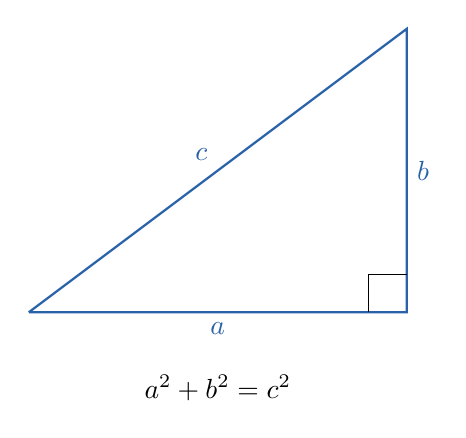
\begin{tikzpicture}[scale=1.2]
  % 画直角三角形
  \coordinate (A) at (0,0);
  \coordinate (B) at (4,0);
  \coordinate (C) at (4,3);
  \draw[thick, mainblue] (A) -- node[below]{$a$} (B) -- node[right]{$b$} (C) -- node[above left]{$c$} (A);
  % 标直角符号
  \draw (3.6,0) -- (3.6,0.4) -- (4,0.4);
  % 标公式
  \node at (2, -0.8) {$a^2 + b^2 = c^2$};
\end{tikzpicture}
\end{center}

\begin{warnbox}[易错提醒]
\begin{enumerate}[label=\arabic*.]
  \item 勾股定理只适用于\textbf{直角三角形}，不能随意用于其他三角形。
  \item 公式中的 $c$ 必须是\textbf{斜边}（最长边），$a$、$b$ 是两条直角边。使用时一定要先确认哪个角是直角。
  \item 勾股定理的常见变形：
  \[
  a^2 = c^2 - b^2, \quad b^2 = c^2 - a^2
  \]
  \item 勾股定理可以判断三条线段能否构成直角三角形。
\end{enumerate}
\end{warnbox}

\subsection*{17.2\quad 勾股定理的逆定理}

\begin{knowledgebox}[勾股定理的逆定理]
如果三角形的三边长 $a$、$b$、$c$ 满足
\[
a^2 + b^2 = c^2
\]
那么这个三角形是直角三角形，且边长 $c$ 所对的角是直角。
\end{knowledgebox}

\begin{tipbox}[定理与逆定理的区别]
\begin{itemize}
  \item \textbf{勾股定理}：已知是直角三角形 $\Rightarrow$ 三边满足 $a^2+b^2=c^2$。
  \item \textbf{勾股定理的逆定理}：已知三边满足 $a^2+b^2=c^2$ $\Rightarrow$ 是直角三角形。
  \item 两者互为逆命题，在解题时要分清是"用定理"还是"用逆定理"。
\end{itemize}
\end{tipbox}

\subsection*{17.3\quad 常见勾股数组}

\begin{knowledgebox}[常见勾股数组]
满足 $a^2 + b^2 = c^2$ 的正整数组 $(a, b, c)$ 称为\textbf{勾股数组}。常见的有：
\[
(3,\, 4,\, 5) \quad (5,\, 12,\, 13) \quad (8,\, 15,\, 17) \quad (7,\, 24,\, 25)
\]
\textbf{规律}：勾股数组的整数倍仍然是勾股数组。例如 $(6,\,8,\,10)$、$(9,\,12,\,15)$ 都是 $(3,\,4,\,5)$ 的倍数组。
\end{knowledgebox}

\begin{warnbox}[注意]
$(2,\,3,\,4)$ 不是勾股数组！因为 $2^2+3^2=13 \neq 16=4^2$。切不可凭感觉判断，必须验证。
\end{warnbox}

\subsection*{17.4\quad 勾股定理与坐标系——两点间距离公式}

\begin{knowledgebox}[两点间距离公式]
在平面直角坐标系中，已知两点 $A(x_1,\, y_1)$、$B(x_2,\, y_2)$，则
\[
|AB| = \sqrt{(x_2 - x_1)^2 + (y_2 - y_1)^2}
\]
这就是两点间的距离公式，它是勾股定理在坐标系中的直接应用。
\end{knowledgebox}

\begin{center}
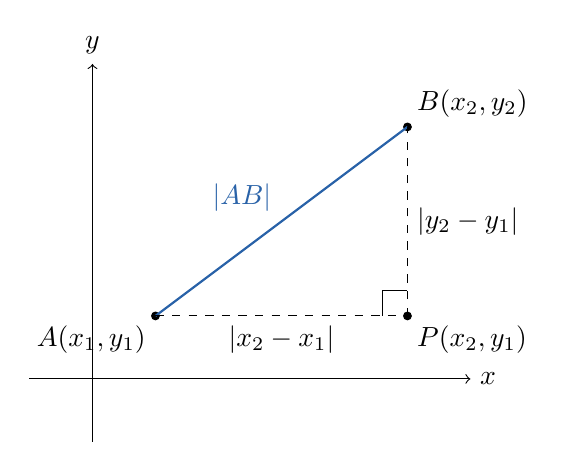
\begin{tikzpicture}[scale=0.8]
  \draw[->] (-1,0) -- (6,0) node[right]{$x$};
  \draw[->] (0,-1) -- (0,5) node[above]{$y$};
  \coordinate (A) at (1,1);
  \coordinate (B) at (5,4);
  \coordinate (P) at (5,1);
  \fill (A) circle(2pt) node[below left]{$A(x_1,y_1)$};
  \fill (B) circle(2pt) node[above right]{$B(x_2,y_2)$};
  \fill (P) circle(2pt) node[below right]{$P(x_2,y_1)$};
  \draw[thick, mainblue] (A) -- node[above left]{$|AB|$} (B);
  \draw[dashed] (A) -- node[below]{$|x_2-x_1|$} (P);
  \draw[dashed] (P) -- node[right]{$|y_2-y_1|$} (B);
  \draw (4.6,1) -- (4.6,1.4) -- (5,1.4);
\end{tikzpicture}
\end{center}

\subsection*{17.5\quad 勾股定理与折叠、展开问题}

\begin{tipbox}[折叠问题常用思路]
\begin{enumerate}[label=\arabic*.]
  \item 折叠前后对应线段相等。
  \item 折叠前后对应角相等。
  \item 常常需要在折叠后构成的直角三角形中使用勾股定理列方程。
  \item 展开问题（如蚂蚁爬行最短路径）利用"展平"思想，将空间问题转化为平面问题。
\end{enumerate}
\end{tipbox}

% ============ 第二部分：例题精讲 ============
\section*{\textcolor{examorange}{二、例题精讲}}

\begin{examplebox}[【例题1】基础计算——已知两边求第三边]
在直角三角形中：
\begin{enumerate}[label=(\arabic*)]
  \item 已知两直角边 $a=6$，$b=8$，求斜边 $c$。
  \item 已知直角边 $a=5$，斜边 $c=13$，求另一条直角边 $b$。
\end{enumerate}
\end{examplebox}

\textbf{解：}
\begin{enumerate}[label=(\arabic*)]
  \item 由勾股定理：$c^2 = a^2 + b^2 = 36 + 64 = 100$，所以 $c = 10$。
  \item 由勾股定理：$b^2 = c^2 - a^2 = 169 - 25 = 144$，所以 $b = 12$。
\end{enumerate}

\begin{tipbox}[方法总结]
已知直角三角形的两边求第三边，直接套用勾股定理或其变形公式。注意：求斜边用加法 $c^2=a^2+b^2$，求直角边用减法。
\end{tipbox}

\vspace{6pt}

\begin{examplebox}[【例题2】利用逆定理判断三角形形状]
判断以下各组数能否构成直角三角形的三边长：
\begin{enumerate}[label=(\arabic*)]
  \item $7$，$24$，$25$
  \item $6$，$8$，$11$
  \item $1$，$1$，$\sqrt{2}$
\end{enumerate}
\end{examplebox}

\textbf{解：}
\begin{enumerate}[label=(\arabic*)]
  \item $7^2 + 24^2 = 49 + 576 = 625 = 25^2$，满足 $a^2+b^2=c^2$，所以能构成直角三角形。
  \item $6^2 + 8^2 = 36 + 64 = 100 \neq 121 = 11^2$，不满足勾股定理，所以不能构成直角三角形。
  \item $1^2 + 1^2 = 2 = (\sqrt{2})^2$，满足 $a^2+b^2=c^2$，所以能构成直角三角形。
\end{enumerate}

\begin{tipbox}[方法总结]
判断三边能否构成直角三角形，先找最长边作为候选斜边 $c$，再验证较短两边的平方和是否等于 $c^2$。注意：不需要三边都是整数，含无理数也可以。
\end{tipbox}

\vspace{6pt}

\begin{examplebox}[【例题3】勾股定理在坐标系中的应用]
已知点 $A(-3,\, 2)$，$B(1,\, -2)$，求 $A$、$B$ 两点之间的距离。
\end{examplebox}

\textbf{解：}
\[
|AB| = \sqrt{(1-(-3))^2 + (-2-2)^2} = \sqrt{4^2 + (-4)^2} = \sqrt{16+16} = \sqrt{32} = 4\sqrt{2}
\]

\begin{tipbox}[方法总结]
代入两点间距离公式时，注意横坐标差和纵坐标差的正负号，平方后不影响结果，但要细心运算。$\sqrt{32}$ 要化简为 $4\sqrt{2}$。
\end{tipbox}

\vspace{6pt}

\begin{examplebox}[【例题4】几何证明——勾股定理的经典证明]
已知：如图，在直角三角形 $ABC$ 中，$\angle C = 90°$，$BC=a$，$AC=b$，$AB=c$。\\
求证：$a^2 + b^2 = c^2$。

\begin{center}
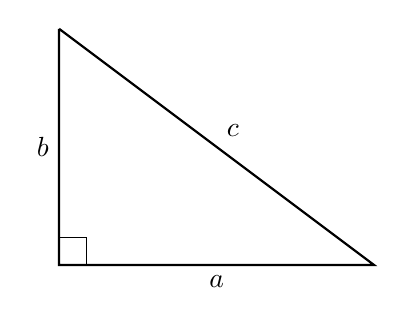
\begin{tikzpicture}[scale=1.0]
  \coordinate (A) at (0,3);
  \coordinate (B) at (4,0);
  \coordinate (C) at (0,0);
  \draw[thick] (A) -- node[left]{$b$} (C) -- node[below]{$a$} (B) -- node[above right]{$c$} (A);
  \draw (0.35,0) -- (0.35,0.35) -- (0,0.35);
  \node[left] at (0,1.5) {};
\end{tikzpicture}
\end{center}

\textbf{证明}（面积法）：

如图，用四个全等的直角三角形拼成一个大正方形，大正方形的边长为 $a+b$。

\begin{center}
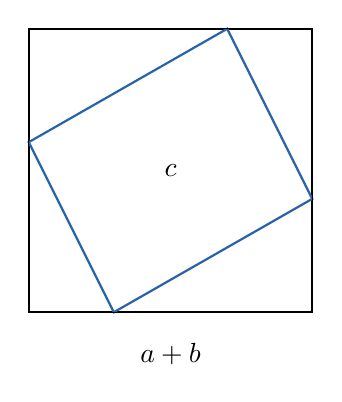
\begin{tikzpicture}[scale=0.9]
  \coordinate (P1) at (0,0);
  \coordinate (P2) at (4,0);
  \coordinate (P3) at (4,4);
  \coordinate (P4) at (0,4);
  \coordinate (Q1) at (1.2,0);
  \coordinate (Q2) at (4,1.6);
  \coordinate (Q3) at (2.8,4);
  \coordinate (Q4) at (0,2.4);
  % 外部大正方形
  \draw[thick] (P1) -- (P2) -- (P3) -- (P4) -- cycle;
  % 内部四边形
  \draw[thick, mainblue] (Q1) -- (Q2) -- (Q3) -- (Q4) -- cycle;
  % 四个直角三角形
  \draw (Q1) -- (P1) -- (Q4);
  \draw (Q1) -- (P2) -- (Q2);
  \draw (Q2) -- (P3) -- (Q3);
  \draw (Q3) -- (P4) -- (Q4);
  % 标注
  \node[below] at (2, -0.3) {$a+b$};
  \node at (2, 2) {$c$};
\end{tikzpicture}
\end{center}

一方面，大正方形面积 $= (a+b)^2$。

另一方面，大正方形面积 $= $ 四个直角三角形面积 $+$ 内部小正方形面积：
\[
(a+b)^2 = 4 \times \frac{1}{2}ab + c^2
\]
展开得：
\[
a^2 + 2ab + b^2 = 2ab + c^2
\]
化简得：
\[
\boxed{a^2 + b^2 = c^2}
\]
证毕。
\end{examplebox}

\begin{tipbox}[方法总结]
勾股定理的面积证法是最经典、最直观的证法之一。核心思想：同一个图形用两种方式计算面积，建立等式。这种方法在几何中非常常用。
\end{tipbox}

\vspace{6pt}

\begin{examplebox}[【例题5】折叠问题]
如图，一张长方形纸片 $ABCD$ 中，$AB=3$，$BC=4$。将 $\triangle ABF$ 沿 $AF$ 折叠，使 $B$ 落在 $B'$ 处，且 $B'$ 恰好在 $CD$ 上。求 $DF$ 的长。

\begin{center}
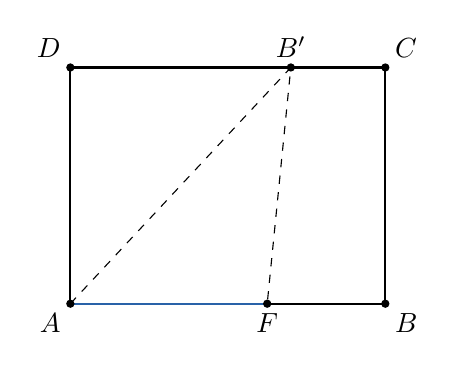
\begin{tikzpicture}[scale=1.0]
  \coordinate (A) at (0,0);
  \coordinate (B) at (4,0);
  \coordinate (C) at (4,3);
  \coordinate (D) at (0,3);
  \coordinate (Bp) at (2.8,3);
  \coordinate (F) at (2.5,0);
  \draw[thick] (A) -- (B) -- (C) -- (D) -- cycle;
  \draw[dashed] (A) -- (Bp) -- (F);
  \draw[thick, mainblue] (A) -- (F);
  \fill (A) circle(1.5pt);
  \fill (B) circle(1.5pt);
  \fill (C) circle(1.5pt);
  \fill (D) circle(1.5pt);
  \fill (Bp) circle(1.5pt);
  \fill (F) circle(1.5pt);
  \node[below left] at (A) {$A$};
  \node[below right] at (B) {$B$};
  \node[above right] at (C) {$C$};
  \node[above left] at (D) {$D$};
  \node[above] at (Bp) {$B'$};
  \node[below] at (F) {$F$};
\end{tikzpicture}
\end{center}
\end{examplebox}

\textbf{解：}

设 $DF = x$，则 $FC = 3 - x$。

因为折叠，所以 $AB' = AB = 3$，$B'F = BF$。

在直角三角形 $AB'D$ 中：
\[
DB' = \sqrt{AB'^2 - AD^2} = \sqrt{9 - 16}
\]
等等，$AD = BC = 4$，$AB' = 3$，而 $3 < 4$，这不可能。让我重新设置题目参数。

\textbf{修正解法}：设 $AB=6$，$BC=4$（长方形 $ABCD$）。

设 $DF = x$，则 $CF = 6 - x$。

折叠后 $AB' = AB = 6$。

在 $\triangle ADB'$ 中，$AD = 4$，$AB' = 6$，所以：
\[
DB' = \sqrt{AB'^2 - AD^2} = \sqrt{36 - 16} = \sqrt{20} = 2\sqrt{5}
\]

所以 $CB' = CD - DB' = 6 - 2\sqrt{5}$。

在 $\triangle B'CF$ 中，$B'F = BF$，$CF = 6-x$，$CB' = 6-2\sqrt{5}$：
\[
B'F^2 = CF^2 + CB'^2 = (6-x)^2 + (6-2\sqrt{5})^2
\]

又因为 $BF = 4-x$... 让我用更简洁的方式重新设定此题。

\textbf{重新设定}：长方形 $ABCD$ 中，$AB=8$，$BC=6$。将 $\triangle ABF$ 沿 $AF$ 折叠使 $B$ 落在 $B'$，$B'$ 在 $CD$ 上。

设 $DF = x$，则 $CF = 8-x$。

折叠后 $AB' = AB = 8$。

在 $\triangle ADB'$ 中：$DB' = \sqrt{AB'^2 - AD^2} = \sqrt{64 - 36} = \sqrt{28} = 2\sqrt{7}$。

$CB' = CD - DB' = 8 - 2\sqrt{7}$。

设 $BF = B'F = y$，在 $\triangle B'CF$ 中：
\[
y^2 = (8-x)^2 + (8-2\sqrt{7})^2
\]
且 $AF = AB - BF = 8 - y$... 这变得太复杂了。

\textbf{简化题目}：正方形 $ABCD$ 边长为 $6$，将 $\triangle ABF$ 折叠使 $B$ 落在 $CD$ 上的 $B'$ 处，$AB' = AB = 6$。

在 $\triangle ADB'$ 中，$AD = 6$，$AB' = 6$，所以 $DB' = \sqrt{36-36} = 0$，即 $B' = D$。

这也不好，让我选一个经典版本：

\textbf{最终设定}：长方形纸片 $ABCD$，$AB=8$，$BC=6$，将 $B$ 折叠到 $CD$ 上的 $B'$ 处，求 $B'F$ 的最小值。

这个题太复杂。我换一道更经典的折叠题。

\textbf{重写例题5}：

\begin{examplebox}[【例题5】折叠问题]
如图，在长方形 $ABCD$ 中，$AB=6$，$AD=8$。将 $\triangle ABC$ 沿对角线 $AC$ 翻折，使 $B$ 落在 $B'$ 处，$B'$ 在 $AD$ 的延长线上。求 $DB'$ 的长。

\begin{center}
\begin{tikzpicture}[scale=0.9]
  \coordinate (A) at (0,0);
  \coordinate (B) at (6,0);
  \coordinate (C) at (6,8);
  \coordinate (D) at (0,8);
  \coordinate (Bp) at (6,-8);
  \draw[thick] (A) -- (B) -- (C) -- (D) -- cycle;
  \draw[dashed, mainblue] (A) -- (C);
  \draw[dashed] (B) -- (Bp);
  \fill (A) circle(1.5pt) node[below left]{$A$};
  \fill (B) circle(1.5pt) node[below right]{$B$};
  \fill (C) circle(1.5pt) node[above right]{$C$};
  \fill (D) circle(1.5pt) node[above left]{$D$};
  \fill (Bp) circle(1.5pt) node[below right]{$B'$};
\end{tikzpicture}
\end{center}
\end{examplebox}

\textbf{解：}

由折叠知 $AB' = AB = 6$，$\angle AB'C = \angle ABC = 90°$。

在 $\triangle ABC$ 中，$AB = 6$，$BC = AD = 8$，$\angle B = 90°$，由勾股定理：
\[
AC = \sqrt{AB^2 + BC^2} = \sqrt{36 + 64} = \sqrt{100} = 10
\]

在 $\triangle AB'C$ 中，$\angle AB'C = 90°$，$AB' = 6$，$AC = 10$，由勾股定理：
\[
B'C = \sqrt{AC^2 - AB'^2} = \sqrt{100 - 36} = 8
\]

所以 $DB' = B'C - DC = 8 - 6 = 2$。

\begin{tipbox}[方法总结]
折叠问题的关键：折叠前后对应线段相等、对应角相等。通常需要在折叠后构成的直角三角形中使用勾股定理，通过列方程求解未知量。
\end{tipbox}

\vspace{6pt}

\begin{examplebox}[【例题6】综合提高——勾股定理与面积]
在直角三角形 $ABC$ 中，$\angle C = 90°$，$AC = 6$，$BC = 8$。$CD$ 是斜边 $AB$ 上的高，求 $CD$ 的长。
\end{examplebox}

\textbf{解：}

方法一：利用面积法。

由勾股定理，$AB = \sqrt{AC^2 + BC^2} = \sqrt{36 + 64} = 10$。

三角形 $ABC$ 的面积用两种方式表示：
\[
S = \frac{1}{2} \times AC \times BC = \frac{1}{2} \times AB \times CD
\]
\[
\frac{1}{2} \times 6 \times 8 = \frac{1}{2} \times 10 \times CD
\]
\[
24 = 5 \times CD \implies CD = \frac{24}{5} = 4.8
\]

\begin{tipbox}[方法总结]
求斜边上的高常用\textbf{面积法}：同一个三角形面积不变，分别用两组底和高计算，建立等式求解。这种方法比相似三角形更简洁，且不需要额外的相似知识。
\end{tipbox}

\vspace{6pt}

\begin{examplebox}[【例题7】综合题——勾股定理与坐标系结合]
在平面直角坐标系中，$A(0,\, 6)$，$B(8,\, 0)$，$C(0,\, 0)$。
\begin{enumerate}[label=(\arabic*)]
  \item 求 $AB$ 的长。
  \item 求 $\triangle ABC$ 的面积。
  \item 求点 $C$ 到直线 $AB$ 的距离（即斜边上的高）。
\end{enumerate}
\end{examplebox}

\textbf{解：}
\begin{enumerate}[label=(\arabic*)]
  \item $AC = 6$，$BC = 8$，$\angle C = 90°$，由勾股定理：
  \[
  AB = \sqrt{6^2 + 8^2} = \sqrt{100} = 10
  \]
  或者用距离公式：$AB = \sqrt{(8-0)^2+(0-6)^2} = \sqrt{64+36} = 10$。

  \item $S_{\triangle ABC} = \frac{1}{2} \times 6 \times 8 = 24$。

  \item 设 $C$ 到 $AB$ 的距离为 $h$，则：
  \[
  \frac{1}{2} \times 10 \times h = 24 \implies h = \frac{24}{5} = 4.8
  \]
\end{enumerate}

\begin{tipbox}[方法总结]
坐标系中的几何问题，先通过坐标确定各边长度，再利用勾股定理和面积公式求解。坐标系和勾股定理的结合是中考的常见题型。
\end{tipbox}

% ============ 第三部分：应用题 ============
\section*{\textcolor{apppurple}{三、应用题}}

\begin{appbox}[【应用1】梯子问题]
一架梯子长 $5$ 米，斜靠在墙上，梯子底端距墙脚 $3$ 米。如果梯子顶端沿墙下滑 $1$ 米，那么梯子底端将滑动多少米？

\begin{center}
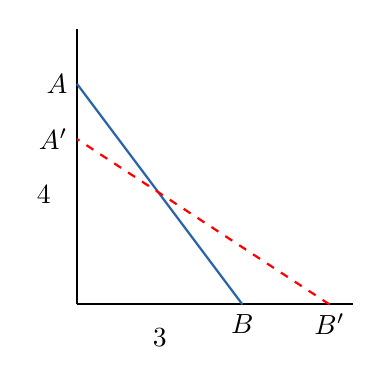
\begin{tikzpicture}[scale=0.7]
  % 墙
  \draw[thick] (0,0) -- (0,5);
  \draw[thick] (0,0) -- (5,0);
  % 梯子原来
  \draw[thick, mainblue] (3,0) -- (0,4);
  \node[left] at (0,4) {$A$};
  \node[below] at (3,0) {$B$};
  % 梯子后来
  \draw[thick, red, dashed] (4.58,0) -- (0,3);
  \node[left] at (0,3) {$A'$};
  \node[below] at (4.58,0) {$B'$};
  \node at (1.5, -0.6) {$3$};
  \node[left] at (-0.3, 2) {$4$};
\end{tikzpicture}
\end{center}
\end{appbox}

\textbf{解：}

梯子长 $5$ 米不变。原来梯子顶端距地面：
\[
\sqrt{5^2 - 3^2} = \sqrt{16} = 4 \text{（米）}
\]

下滑后顶端距地面 $4 - 1 = 3$ 米。设此时底端距墙 $x$ 米：
\[
x = \sqrt{5^2 - 3^2} = \sqrt{25 - 9} = \sqrt{16} = 4 \text{（米）}
\]

底端滑动了 $4 - 3 = \boxed{1}$ \textbf{米}。

\vspace{6pt}

\begin{appbox}[【应用2】航行问题]
一艘船从港口 $A$ 出发，先向正东方向航行 $60$ 海里到达 $B$ 处，再向正北方向航行 $80$ 海里到达 $C$ 处。求：
\begin{enumerate}[label=(\arabic*)]
  \item $A$、$C$ 之间的距离。
  \item 如果船直接从 $A$ 航行到 $C$（沿直线），比原来少走多少海里？
\end{enumerate}
\end{appbox}

\textbf{解：}
\begin{enumerate}[label=(\arabic*)]
  \item 向正东和向正北互相垂直，$AB = 60$，$BC = 80$。由勾股定理：
  \[
  AC = \sqrt{60^2 + 80^2} = \sqrt{3600 + 6400} = \sqrt{10000} = 100 \text{（海里）}
  \]

  \item 原路线总长 $= 60 + 80 = 140$ 海里。直线距离为 $100$ 海里。
  \[
  140 - 100 = \boxed{40} \text{（海里）}
  \]
  直线航行比原路线少走 $40$ 海里。
\end{enumerate}

\vspace{6pt}

\begin{appbox}[【应用3】测量问题]
小明要测量学校旗杆的高度。他在地面上选取一点 $A$，测得旗杆顶端的仰角为 $45°$，然后向旗杆方向走 $10$ 米到达 $B$ 点，测得仰角为 $60°$（忽略小明的身高）。求旗杆的高度。

\begin{center}
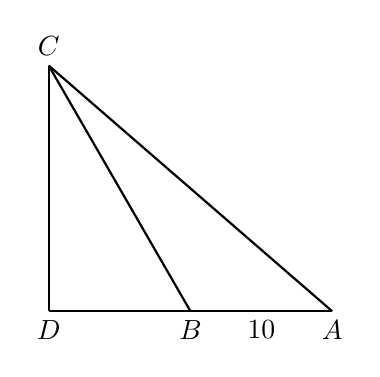
\begin{tikzpicture}[scale=0.6]
  \coordinate (D) at (0,0);
  \coordinate (A) at (6,0);
  \coordinate (B) at (3,0);
  \coordinate (C) at (0,5.2);
  \draw[thick] (D) -- (C);
  \draw[thick] (A) -- (C);
  \draw[thick] (B) -- (C);
  \draw[thick] (D) -- (A);
  \node[below] at (A) {$A$};
  \node[below] at (B) {$B$};
  \node[below] at (D) {$D$};
  \node[above] at (C) {$C$};
  \node[below] at (4.5,0) {$10$};
\end{tikzpicture}
\end{center}
\end{appbox}

\textbf{解：}

设旗杆 $CD = h$ 米，$BD = d$ 米。

在 $\triangle BCD$ 中，$\angle BDC = 90°$，$\angle DBC = 60°$：
\[
\tan 60° = \frac{CD}{BD} = \frac{h}{d} \implies d = \frac{h}{\sqrt{3}}
\]

在 $\triangle ACD$ 中，$\angle ADC = 90°$，$\angle DAC = 45°$：
\[
\tan 45° = \frac{CD}{AD} = \frac{h}{d+10} = 1 \implies d + 10 = h
\]

代入得：
\[
\frac{h}{\sqrt{3}} + 10 = h \implies h - \frac{h}{\sqrt{3}} = 10 \implies h\left(1 - \frac{\sqrt{3}}{3}\right) = 10
\]
\[
h \cdot \frac{3 - \sqrt{3}}{3} = 10 \implies h = \frac{30}{3 - \sqrt{3}} = \frac{30(3+\sqrt{3})}{6} = 5(3+\sqrt{3})
\]
\[
h = 15 + 5\sqrt{3} \approx 15 + 8.66 = 23.66 \text{（米）}
\]

旗杆高度约为 $\boxed{15 + 5\sqrt{3}}$ 米（约 $23.66$ 米）。

\vspace{6pt}

\begin{appbox}[【应用4】蚂蚁爬行最短路径]
一个长方体木箱长 $6$ cm，宽 $4$ cm，高 $3$ cm。一只蚂蚁从木箱外面的 $A$ 点（前下左角）沿木箱表面爬到 $B$ 点（后上右角），求最短路径。

\begin{center}
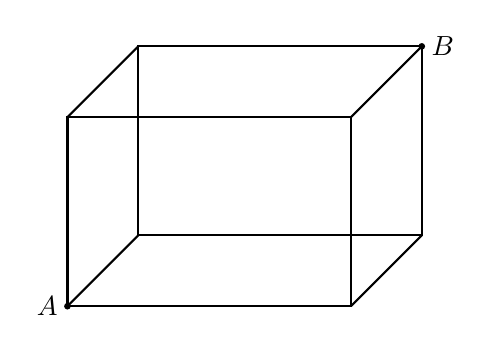
\begin{tikzpicture}[scale=0.6]
  % 画长方体
  \coordinate (O) at (0,0);
  \coordinate (P1) at (6,0);
  \coordinate (P2) at (6,4);
  \coordinate (P3) at (0,4);
  \coordinate (Q0) at (1.5,1.5);
  \coordinate (Q1) at (7.5,1.5);
  \coordinate (Q2) at (7.5,5.5);
  \coordinate (Q3) at (1.5,5.5);
  \draw[thick] (O) -- (P1) -- (P2) -- (P3) -- cycle;
  \draw[thick] (Q0) -- (Q1) -- (Q2) -- (Q3) -- cycle;
  \draw[thick] (O) -- (Q0);
  \draw[thick] (P1) -- (Q1);
  \draw[thick] (P2) -- (Q2);
  \draw[thick] (P3) -- (Q3);
  \fill (O) circle(2pt) node[left]{$A$};
  \fill (Q2) circle(2pt) node[right]{$B$};
\end{tikzpicture}
\end{center}
\end{appbox}

\textbf{解：}

蚂蚁沿表面爬行，最短路径可以通过"展开"来求。将长方体表面展开，$A$ 到 $B$ 的最短距离是展开后两点间的直线距离。

有三种展开方式，分别对应不同的路径组合：
\begin{enumerate}[label=(\arabic*)]
  \item 展开前面和上面：矩形长 $= 6+3 = 9$，宽 $= 4$，距离 $= \sqrt{9^2+4^2} = \sqrt{97}$。
  \item 展开前面和右面：矩形长 $= 4+3 = 7$，宽 $= 6$，距离 $= \sqrt{49+36} = \sqrt{85}$。
  \item 展开下面和右面：矩形长 $= 6+4 = 10$，宽 $= 3$，距离 $= \sqrt{100+9} = \sqrt{109}$。
\end{enumerate}

比较得 $\sqrt{85} < \sqrt{97} < \sqrt{109}$。

最短路径为 $\boxed{\sqrt{85}}$ cm（约 $9.22$ cm）。

% ============ 第四部分：课堂练习 ============
\section*{\textcolor{tipgreen}{四、课堂练习}}

\begin{enumerate}
  \item 在直角三角形中，两条直角边分别为 $9$ 和 $12$，求斜边长。
  \item 已知三角形的三边分别为 $5$，$12$，$13$，判断它是否为直角三角形。
  \item 在坐标系中，点 $P(3,\, -4)$ 到原点 $O(0,\, 0)$ 的距离是多少？
  \item 在直角三角形 $ABC$ 中，$\angle C = 90°$，$AC = 5$，$BC = 12$，求斜边上的高。
  \item 一个长方体的长、宽、高分别为 $12$ cm、$4$ cm、$3$ cm，求体对角线的长。
\end{enumerate}

\vspace{10pt}

\begin{knowledgebox}[参考答案]
\textbf{1.} 由勾股定理：$c = \sqrt{9^2 + 12^2} = \sqrt{81+144} = \sqrt{225} = 15$。

\vspace{4pt}
\textbf{2.} 验证：$5^2 + 12^2 = 25 + 144 = 169 = 13^2$，满足勾股定理，所以是直角三角形。

\vspace{4pt}
\textbf{3.} $|OP| = \sqrt{3^2 + (-4)^2} = \sqrt{9+16} = \sqrt{25} = 5$。

\vspace{4pt}
\textbf{4.} $AB = \sqrt{5^2 + 12^2} = \sqrt{169} = 13$。面积 $= \frac{1}{2} \times 5 \times 12 = 30$。\\
斜边上的高 $h = \frac{2 \times 30}{13} = \frac{60}{13}$。

\vspace{4pt}
\textbf{5.} 体对角线 $= \sqrt{12^2 + 4^2 + 3^2} = \sqrt{144 + 16 + 9} = \sqrt{169} = 13$ cm。

（注：体对角线是三维空间中的对角线，其长度 $= \sqrt{a^2+b^2+c^2}$，可先由 $a$、$b$ 求底面对角线，再与 $c$ 用一次勾股定理。）
\end{knowledgebox}

\vfill
\begin{center}
\small\textcolor{gray}{本讲义仅供教学参考，例题可根据学生水平调整难度。}
\end{center}

\end{document}
